%%%%%%%%%%%%%%%%%%%%%%%%%%%%%%%%%%%%%%%%%%%%%%%%%%%
\begin{frame}

  \frametitle{AMI database}
  The AMI Meeting Corpus consists of:
  \begin{center}
    \begin{itemize}
      \item 100 hours of meeting recordings
      \item Include close-talking and far-field microphones
      \item Individual and room-view video cameras
      \item Output from a slide projector and an electronic whiteboard
    \end{itemize}
  \end{center}
The meetings were recorded in English using three different rooms with different acoustic properties, and include mostly non-native speakers$^1$.
\footnotetext[1]{\textit{http://groups.inf.ed.ac.uk/ami/corpus/overview.shtml}}

\end{frame}

%%%%%%%%%%%%%%%%%%%%%%%%%%%%%%%%%%%%%%%%%%%%%%%%%%%

\begin{frame}

  \frametitle{AMI database}
  The AMI Meeting Corpus Annotations:
  \begin{center}
    \begin{itemize}
      \item Linguistic (covering all recordings)
        \begin{itemize}
          \item high quality, manually produced orthographic transcription for each individual speaker
          \item word-level timings
        \end{itemize}
      \item behaviours (limited coverage)
        \begin{itemize}
          \item dialogue acts
          \item word-level timings, topic segmentation
          \item extractive and abstractive summaries
          \item the types of head gesture, hand gesture, and gaze direction
          \item movement around the room
          \item emotional state
        \end{itemize}      
    \end{itemize}
  \end{center}
  
\end{frame}

%%%%%%%%%%%%%%%%%%%%%%%%%%%%%%%%%%%%%%%%%%%%%%%%%%%

\begin{frame}

  \frametitle{Advantages}
  \begin{itemize}
    \item Released under a Creative Commons Attribution ShareAlike Licence, similar to the GNU (General Public License).
    \item All of the annotations provided are in one consistent format that represents not just the timecourse of the annotations, but also how they    relate structurally to the transcription and to other annotations
    \item Around $1/3$ of the data is natural and the rest is controlled (role playing)
  \end{itemize}
That would allow us todevelop new techniques on the controlled data first and then begin to test their generalizability using the natural material
\end{frame}

\footnotetext[1]{\textit{http://corpus.amiproject.org}}

%%%%%%%%%%%%%%%%%%%%%%%%%%%%%%%%%%%%%%%%%%%%%%%%%%%

\begin{frame}
    \frametitle{Amicorpus directory}
    \begin{center}
      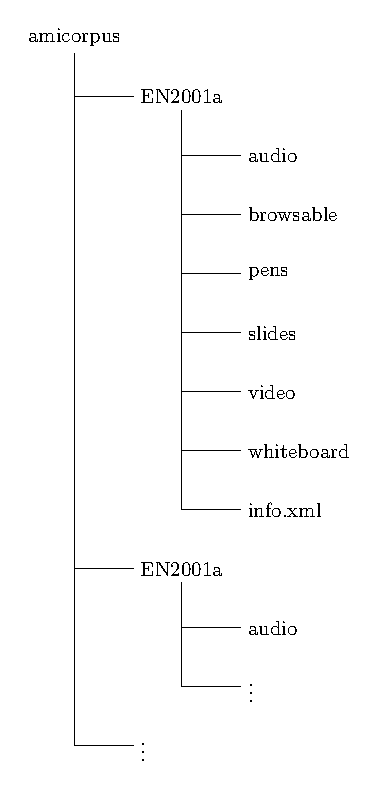
\includegraphics[height=0.6\textheight]{graphics/tree_amicorpus}
    \end{center}
\end{frame}

%%%%%%%%%%%%%%%%%%%%%%%%%%%%%%%%%%%%%%%%%%%%%%%%%%%

\begin{frame}
    \frametitle{Amicorpus IDs and annotations example}
    \begin{itemize}
    \item AMI Corpus Meeting IDs: [IETB][SNB][1-5][0-9][0-9][0-9][a-z]
    \item AMI Corpus Participant IDs: [MF][IET][EDO][0-9][0-9][0-9]
    \end{itemize}
    \begin{center}
      \includegraphics[height=0.4\textheight]{graphics/segments_annotations}
    \end{center}  
    
\end{frame}

